%%%%%%%%%%%%%%%%%%%%%%%%%%%%%%%%%%%%%%%%%%%%%%%%%%%%%%%%%%%%%%%%%%%%%%%%%%%%%
%%%
%%% File: thesis.tex, version 1.9, May 2016
%%%
%%% =============================================
%%% This file contains a template that can be used with the package
%%% cs.sty and LaTeX2e to produce a thesis that meets the requirements
%%% of the Computer Science Department from the Technical University of Cluj-Napoca
%%%%%%%%%%%%%%%%%%%%%%%%%%%%%%%%%%%%%%%%%%%%%%%%%%%%%%%%%%%%%%%%%%%%%%%%%%%%%

\documentclass[12pt,a4paper,twoside]{report}         
\usepackage{cs}              
\usepackage{times}
\usepackage{graphicx}
\usepackage{latexsym}
\usepackage{amsmath,amsbsy}
\usepackage{amssymb}
\usepackage[matrix,arrow]{xy}
\usepackage[T1]{fontenc}
\usepackage{ae,aecompl}
%\usepackage{shortcut} %definitii pentru diacritice; 
\usepackage{amstext}
\usepackage{graphics}
\usepackage{ae,aecompl}
\usepackage{algorithm}
%\usepackage{algorithmic}
\usepackage{color}
\usepackage{enumitem}

% \mastersthesis
\diplomathesis
% \leftchapter
\centerchapter
% \rightchapter
\singlespace
% \oneandhalfspace
% \doublespace

\newcommand{\applicationTitle}{Meal Menu Generator}

\renewcommand{\thesisauthor}{Firstname LASTNAME}    %% Your name.
\renewcommand{\thesismonth}{June}     %% Your month of graduation.
\renewcommand{\thesisyear}{2018}      %% Your year of graduation.
\renewcommand{\thesistitle}{LICENSE THESIS TITLE} 
\renewcommand{\thesissupervisor}{scientific title Firstname LASTNAME}
\newcommand{\department}{\bf FACULTY OF AUTOMATION AND COMPUTER SCIENCE\\
COMPUTER SCIENCE DEPARTMENT}
\newcommand{\thesis}{LUCRARE DE LICEN'T'A}
\newcommand{\utcnlogo}{
\includegraphics[width=15cm]{img/tucn.jpg}}

\newcommand{\uline}[1]{\rule[0pt]{#1}{0.4pt}}
%\renewcommand{\thesisdedication}{P\u{a}rin\c{t}ilor mei}

\begin{document}
%\frontmatter
%\pagestyle{headings}

\newenvironment{definition}[1][Defini\c{t}ie.]{\begin{trivlist}
\item[\hskip \labelsep {\bfseries #1}]}{\end{trivlist}}



%\thesistitle                    %% Generate the title page.
%\authordeclarationpage                %% Generate the declaration page.

\pagenumbering{arabic}
\setcounter{page}{4}



\begin{center}
\utcnlogo

\department

\vspace{4cm}

{\bf \thesistitle} %LICENSE THESIS TITLE}

\vspace{1.5cm}

LICENSE THESIS

\vspace{6cm}

Graduate: {\bf Adrian BIRLADEANU}

Supervisor: {\bf \thesissupervisor}

\vspace{3cm}
{\bf \thesisyear}
\end{center}

\thispagestyle{empty}
\newpage

\begin{center}
\utcnlogo

\department

\end{center}
\vspace{0.5cm}

%\begin{small}
\begin{tabular}{p{7cm}p{8cm}}
 %\hspace{-1cm}& APPROVED,\\
 \hspace{-1cm}DEAN, & HEAD OF DEPARTMENT,\\
 \hspace{-1cm}{\bf Prof. dr. eng. Liviu MICLEA} & {\bf Prof. dr. eng. Rodica POTOLEA}\\  
\end{tabular}
 
\vspace{2cm}

\begin{center}
Graduate: {\bf \thesisauthor}

\vspace{1cm}

{\bf \thesistitle}
\end{center}

\vspace{1cm}

\begin{enumerate}
 \item {\bf Project proposal:} {\it Short description of the license thesis and initial data}
\item {\bf Project contents:} {\it (enumerate the main component parts) Presentation page, advisor's evaluation, title of chapter 1, title of chapter 2, ..., title of chapter n, bibliography, appendices.}
\item {\bf Place of documentation:} {\it Example}: Technical University of Cluj-Napoca, Computer Science Department
\item {\bf Consultants:}
\item {\bf Date of issue of the proposal:} November 1, 2016
\item {\bf Date of  delivery:} February 21, 2018 {\it (the date when the document is submitted)}
  \end{enumerate}
\vspace{1.2cm}

\hspace{6cm} Graduate: \uline{6cm} 

\vspace{0.5cm}
\hspace{6cm} Supervisor: \uline{6cm} 
%\end{small}

\thispagestyle{empty}


\newpage
$ $
%\begin{center}
%\utcnlogo

%\department
%\end{center}

\thispagestyle{empty}
\newpage

\begin{center}
\utcnlogo

\department
\end{center}

\vspace{0.5cm}

\begin{center}
{\bf
Declara\c{t}ie pe proprie r\u{a}spundere privind\\ 
autenticitatea lucr\u{a}rii de licen\c{t}\u{a}}
\end{center}
\vspace{1cm}



Subsemnatul(a) \\
\uline{14.8cm}, 
legitimat(\u{a}) cu \uline{4cm} seria \uline{3cm} nr. \uline{4cm}\\
CNP \uline{9cm}, autorul lucr\u{a}rii \uline{2.8cm}\\
\uline{16cm}\\
\uline{16cm}\\
elaborat\u{a} \^{\i}n vederea sus\c{t}inerii examenului de finalizare a studiilor de licen\c{t}\u{a} la Facultatea de Automatic\u{a} \c{s}i Calculatoare, Specializarea \uline{7cm} din cadrul Universit\u{a}\c{t}ii Tehnice din Cluj-Napoca, sesiunea \uline{4cm} a anului universitar \uline{3cm}, declar pe proprie r\u{a}spundere, c\u{a} aceast\u{a} lucrare este rezultatul propriei activit\u{a}\c{t}i intelectuale, pe baza cercet\u{a}rilor mele \c{s}i pe baza informa\c{t}iilor ob\c{t}inute din surse care au fost citate, \^{\i}n textul lucr\u{a}rii \c{s}i \^{\i}n bibliografie.

Declar, c\u{a} aceast\u{a} lucrare nu con\c{t}ine por\c{t}iuni plagiate, iar sursele bibliografice au fost folosite cu 
respectarea legisla\c{t}iei rom\^{a}ne \c{s}i a conven\c{t}iilor interna\c{t}ionale privind drepturile de autor.

Declar, de asemenea, c\u{a} aceast\u{a} lucrare nu a mai fost prezentat\u{a} \^{\i}n fa\c{t}a unei alte comisii de examen de licen\c{t}\u{a}.

\^{I}n cazul constat\u{a}rii ulterioare a unor declara\c{t}ii false, voi suporta sanc\c{t}iunile administrative, respectiv, \emph{anularea examenului de licen\c{t}\u{a}}.

\vspace{1.5cm}

Data \hspace{8cm} Nume, Prenume

\vspace{0.5cm}

\uline{3cm} \hspace{5cm} \uline{5cm}

\vspace{0.5cm}
\hspace{9.4cm}Semn\u{a}tura

\thispagestyle{empty}

\newpage


%\listoftables
%\listoffigures

%\clearpage 
%\newpage

%\begin{comment}
{\color{red}{\bf De citit \^{\i}nainte} (aceast\u{a} pagin\u{a} se va elimina din versiunea final\u{a})}:
\begin{enumerate}
 \item Cele trei pagini anterioare (foaie de cap\u{a}t, foaie sumar, declara\c{t}ie) se vor lista pe foi separate (nu fa\c{t}\u{a}-verso), fiind incluse \^{\i}n lucrarea listat\u{a}. 
 Foaia de sumar (a doua) necesit\u{a} semn\u{a}tura absolventului, respectiv a coordonatorului.
 Pe declara\c{t}ie se trece data c\^{a}nd se pred\u{a} lucrarea la secretarii de comisie.
 \item Pe foaia de cap\u{a}t, se va trece corect titulatura cadrului didactic \^{\i}ndrum\u{a}tor, \^{\i}n englez\u{a} (consulta\c{t}i pagina de unde a\c{t}i desc\u{a}rcat acest document pentru lista cadrelor didactice cu titulaturile lor).
 \item Documentul curent {\bf nu} a fost creat \^{\i}n MS Office. E posibil sa fie mici diferen\c{t}e de formatare. 
\item Cuprinsul \^{\i}ncepe pe pagina nou\u{a}, impar\u{a} (dac\u{a} se face listare fa\c{t}\u{a}-verso), prima pagin\u{a} din capitolul \emph{Introducere} tot a\c{s}a, fiind numerotat\u{a} cu 1. % Pentru actualizarea cuprinsului, click dreapta pe cuprins (zona cuprinsului va apare cu gri), Update field-$>$Update entire table.
\item E recomandat s\u{a} vizualiza\c{t}i acest document \c{s}i \^{\i}n timpul edit\u{a}rii lucr\u{a}rii. % după ce activaţi vizualizarea simbolurilor ascunse de formatare (apăsaţi simbolul  din Home/Paragraph).
\item Fiecare capitol \^{\i}ncepe pe pagin\u{a} nou\u{a}. % datorită simbolului ascuns Section Break (Next Page) care este deja introdus la capitolul precedent. Dacă ştergeţi din greşeală simbolul, se reintroduce (Page Layout -> Breaks).
\item Folosi\c{t}i stilurile predefinite (Headings, Figure, Table, Normal, etc.)
\item Marginile la pagini nu se modific\u{a}.
\item Respecta\c{t}i restul instruc\c{t}iunilor din fiecare capitol.
\end{enumerate}
 
%\end{comment}

\newpage

\tableofcontents
\newpage




%\subsection{Subsection}
%%Each table used in this document is labeled as Table x.y, where x represents the chapter number, and y shows the table number within the current chapter. Leave a blank line between and after each table, relative to the adjacent paragraphs (table~\ref{table:nonlin}).
%
%\begin{table}[ht]
%\caption{Nonlinear Model Results}
%\centering                          % tabel centrat
%\begin{tabular}{|c|c|c|c|}          % 4 coloane centrate
%\hline\hline                        % linie orizontala dubla
%Case & Method\#1 & Method\#2 & Method\#3 \\ [0.5ex]   % inserare tabel
%%heading
%\hline                              % linie orizontal simpla
%1 & 50 & 837 & 970 \\               % corpul tabelului
%2 & 47 & 877 & 230 \\
%3 & 31 & 25 & 415 \\[1ex]           % [1ex] adds vertical space
%\hline
%\end{tabular}
%  % titlul tabelului
%\label{table:nonlin}                % \label{table:nonlin} introduce eticheta folosita pentru referirea tabelului in text; referirea in text se va face cu \ref{table:nonlin}
%\end{table}
%
%Each figure used in the document must be cited within the text (ex: in figure x.y the system components are presented... ) and labeled. The labeling must be as Figure x.y where x represents the chapter number, and y shows the number of the figure within the current chapter.
% E.g.: figure \ref{fig:imag}.
%
%\begin{figure}[ht]
%    \centering
%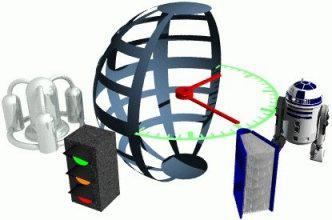
\includegraphics[]{img/test.jpg}
%    \caption{The figure`s name}
%    \label{fig:imag}
%\end{figure}
%
%Each chapter must start on a new page.

\usepackage{graphicx}


\chapter{Introduction - Project Context}
\label{ch:introduction}
\pagestyle{headings}

\section{Project context}
\label{sec:introduction-context}

\subsection{General Context}
\label{subsec:introduction-general-context}
With the increase of internet speed across the globe, possible among others to the appearance of 5G networks and, in
the near future, to the SpaceX Starlink network, it is now possible to stream increasingly larger data across the
internet. \
According to .., \ % todo: insert reference https://www.speedtest.net/global-index#mobile
the global mobile internet speed was of about 31Mbps for download and 11.88Mbps for upload. \
Although these values are still pretty low, they are bound to improve in the near future.
The highest values were achieved using 4G LTE and 4G LTE-A networks.

\begin{table}[ht]
    \caption{Average internet speed}
    \centering
    \begin{tabular}{|c|c|c|}
        \hline\hline
        Rank & Country & Download speed \[Mbps\] \\ [0.5ex]
        \hline
        1 & South Korea & 117.79 \\
        2 & Qatar & 77.07  \\
        3 & Norway & 72.80 \\
        4 & UAE & 69.72 \\
        5 & Australia & 68.87 \\
        6 & Canada & 67.57 \\
        7 & Netherlands & 62.86 \\
        8 & Croatia & 59.83 \\
        9 & China & 58.33 \\
        10 & Switzerland & 57.09 \\
        40 & Romania & 37.76
    \end{tabular}
    \label{table:internetSpeed}
\end{table}

% todo: mention ml/deep learning

\subsection{5G}
\label{subsec:5g}
According to ..\ % todo: quote https://www.telekom.com/en/company/details/5g-speed-is-data-transmission-in-real-time-544498
5G internet speeds should reach speeds of about 10Gbps, enough to stream video-audio in real time.
However, according to .. \ % todo: quote https://www.forbes.com/sites/bobodonnell/2019/11/22/real-world-5g-speeds/#3ec794804f96
and ..,\ % todo: quote https://5g.co.uk/guides/how-fast-is-5g/
such speeds cannot be reached with the current infrastructure, with download speeds averaging at about 130Mbps-240Mbps, \
with peaks at about 600Mbps.
However, certain variants have reached peaks of 1.8 Gbps (using mmWave 5G services) and event 1Tbps in controlled \
test environments.

It must be noted that these are only the early days of 5G networks, and that in the coming years these speeds are \
bound to improve.

According to .. \ % todo: quote https://web.archive.org/web/20190419231844/http://www.5gamericas.org/files/5115/4169/8314/5G_Americas_URLLLC_White_Paper_Final_11.8.pdf , https://en.wikipedia.org/wiki/5G
possible use cases for 5G networks include but are not limited to  Smart Factories (industrial control, robot control),\
 healthcare (remote diagnosis and surgery), entertainment (immersive entertainment, online gaming), transport \
industry (driver assistance, enhanced safety, autonomous driving, traffic management), energy sector (smart energy, \
smart grid).


\subsection{Satellite internet}
\label{subsec:satellite-internet}
As mentioned in .., \ % todo: quote https://www.forbes.com/sites/bobodonnell/2019/11/22/real-world-5g-speeds/#3ec794804f96
for 5G, the radio wave internet speed is inversely proportional to the distance covered. \
This means that regular 5G high speed internet will probably be limited to regions densely and medium populated and \
to research outposts because of infrastructure costs. \
A valid alternative for sparsely populated areas would be satellite internet. \
Several US companies have already begun taking steps towards a commercial solution. \
The most notable player is SpaceX with its project, Starlink, a network of several dozen thousands satellites in lower \
Earth orbit, in the range of 350\-550 km from Earth, as opposed to the average altitude of \
1000+ km for satellites in lower earth orbit. \
According to .. , % todo: quote https://www.pcmag.com/news/371511/spacexs-satellite-internet-plans-for-mid-2020-launch-in-the
the desired average speed is about 1Gbps. \
 .. % todo: quote https://spacenews.com/spacex-launches-second-batch-of-starlink-broadband-satellites/
mentions that tests with the US military achieved peak speeds of around 610 Mbps, while the network isn't fully \
functional yet, with thousands of satellites still to be sent to space. \
The official \href{https://www.starlink.com/}{Starlink} website it expects to reach coverage for northern US and \
Canada by 2020, and for the rest of the world by 2021.\
Other companies, including Amazon and OneWeb, have started work on deploying their own internet satellite network.

\subsection{Motivation}
\label{subsec:introduction-motivation}
With the rise of 5G internet and satellite-based internet, it will be increasingly easier to stream real-time data \
from one place in the world to another place on the opposite side. \
One use case for this increase in speed is the development of commercial drones controlled remotely over the internet.\
With 5G's speed, bandwidth and latency, it will be possible for a robot to transmit in virtually real-time audio-video \
data to a remote operator and to receive control commands from that operator.

\begin{figure}[ht]
    \label{fig:overview1}
    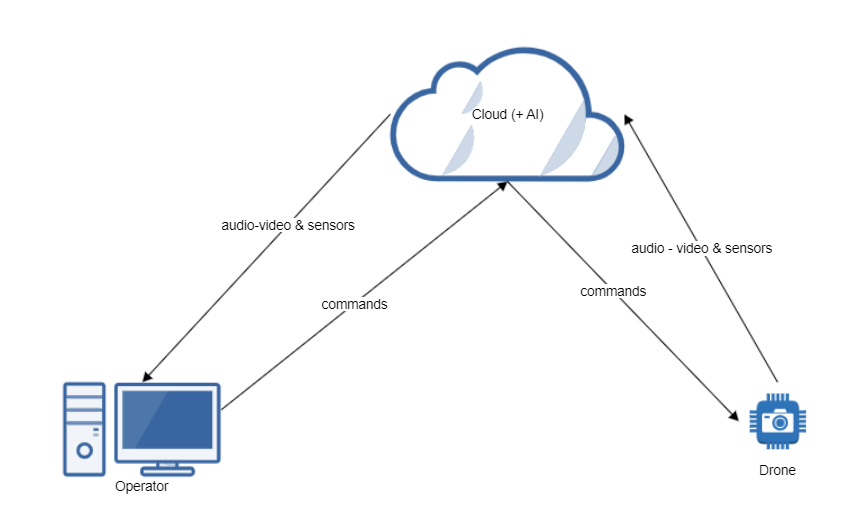
\includegraphics[width=15cm, height=10cm, keepaspectratio]{img/overview1.PNG}
    \caption{High Level Overview}
\end{figure}

This use case can be extended to autonomous robots. \
Instead of adding considerable computation capabilities to a robot (CPU, memory, GPU) os that it can run an AI, the \
robot could be fitted with minimal hardware designed only to transmit audio-video and receive commands from an AI that \
runs in the cloud. \
This way, if any malfunction occurs on the robot, the equipment could be easily replaced with lower costs because the \
equipment used was a lot cheaper than it would have been if hardware had to run the AI . \
Another option would be to use dedicated hardware that puts an emphasis on durability and can properly function in \
a wide range of conditions (rain, extreme low/high temperatures). \
Additionally, this type of setup would also use less energy in order to run, thus extending battery life and allowing \
higher autonomy.




\usepackage{graphicx}


\chapter{Project Objectives and Specifications}
\label{ch:specification}

\section{Problem specification}
\label{sec:specification-specification}

Following a healthy diet is a difficult task even to young people, and especially so for elder people. \
One must keep \
track of all the nutrients and calories of what they eat and cook and compare them to some reference values. \
The reference \
can be taken from a specialized doctor/nutritionist, but most of the time it's taken from the internet. \
It is even more \
difficult for older people, who may lack the mobility to search for what they need or even read the finely printed ingredients.

This task can be made easier using specialized software. \
However, this isn't a new idea and there are already \
plenty of web and mobile application designed to \
generate menus and meals, but most of them are somewhat incomplete. \
Most of the time, they do not take into account all possible \
variables, such as specific diseases, possible allergies, level of physical activity. \
Another problem is that since \
these applications are available online for anyone, the results are not validated by an experienced professional, such \
as a nutritionist or a family doctor. \
Therefore, these menus can end up doing more harm than good.

Another aspect about the available web applications is that they generate general menus, sometimes even without a recipe,
without taking into account any \
geographic or cultural aspects or even available local products. \
The users end up having to search for the right ingredients \
in order to cook the meals, sometimes not even finding them in their region. \
Even more, users need to spend some time \
cooking these meals, which is even more time consuming.

After having analyzed all the above aspects, I have decided to design and implement the \
\applicationTitle{} in order to fix these issues, thus making the users' lives easier and allowing them to \
focus on other aspects of life that are more enjoyable than eating healthy.


\section{General Objectives}
\label{sec:specification-objectives}
As stated above, the primary objective of \applicationTitle{} is to create a menu generator application that can solve \
most of the problems of the other existing alternatives. \
This will allow older people to maintain a healthy diet by offering them recommendations for meals for the entire day.

In order to accomplish its purpose, the application needs to gather a certain amount of information about \
each user. \
This includes personal information (age, gender, weight, height, physical activity level). \
In addition \
to this the system also requires information about specific allergies (in order to exclude certain foods when generating \
a menu) and about current chronic diseases (so that a nutritionist will be aware of them when validating the user \
profile). \
Using the information above, a profile is generated that include the body mass index (used to determine if a \
person is normal weight, underweight, overweight or obese) and recommended nutrient, caloric, vitamin and mineral intake \
for a day. \
The recommended daily nutritional intake levels represent the amount of nutrients that are sufficient in order \
to meet the requirements of 97\-98\% of healthy people. \
However, no menu can be generated until the profile is reviewed \
by a nutritionist.

The information presented above will be the input to a choice-based algorithm that will generated an optimal recommendation for a \
menu for a day. \
The other inputs will include certain non-functional requirements (preferred price, delivery time, geographical \
location of vendor). \
Since one of the objectives of this system is to generated meals that can be delivered to the users' homes, \
the system will require extensive information about local sellers. \
This will include, along information about geographical \
location, information about the meals they offer(type, price, cooking time, ingredients, nutritional values, weight). \
This will require food vendors to have dedicated accounts in the system in order to edit their company's offers. \
Using all \
this information, an algorithm will compute the best possible menu to satisfy an elder's nutritional \
daily intake requirements and non-functional requirements. \
A use case diagram can be seen in figure 2.1 \ref{fig:usecase1}.
A basic activity flow can be seen in diagram 2.2.

\begin{figure}[ht]
    \label{fig:usecase1}
    %\centering
    \includegraphics[width=15cm, height=50cm,keepaspectratio]{staruml/UseCaseDiagram1.png}
    \caption{Use Case Diagram}
\end{figure}

\begin{figure}[ht]
    \label{fig:activity1}
    %\centering
    \includegraphics[width=15cm, height=50cm,keepaspectratio]{staruml/ActivityDiagram1.png}
    \caption{Use Case Diagram}
\end{figure}

However, all the information above leads to a very large search space, possibly leading to performance issues. \
This makes an exhaustive search very time consuming, since there are very many possible combinations. \
The users desire a fast way to \
generate menus, especially if they don't like one of the menus generated and want to generate another one. \
This is why I have decided to use a choice-function based hyper heuristic\
\footnote{A high level hyper heuristic that applies other, low level heuristics on a search space}.


\section{Functional Requirements}
\label{sec:specification-functional}

In software engineering, a functional requirement is a function of a system or its components. \
Such a function consists of a specific set of inputs, a behavior and an output. \
Functional requirements describe what the system \
is expected to do in order to accomplish its purpose and reach the desired results.

The functional requirements I have set out to achieve are mosyly based on the general objectives presented above.\
First, the application requires extensive information about various food vendors and their offers, alongside some \
personal information about the elder users. \
Once the user data is in the database, the application should be able \
to generate user profiles describing the recommended daily nutritional values.

Ideally, there would be 3 types of users: elders, nutritionists and food distributors, each having to log in \
into the application. \
An elder should be able to edit his contact information, his personal health information, choose his nutritionist, \
generate a menu for \
a day and view the menu's properties (nutritional values). \
A nutritionist should be able to view the elders who \
have chosen him as their nutritionist, view the elder's personal information, edit the recommended nutritional \
intake values and validate a certain user profile. \
An elder cannot create a menu until his profile has been validated by a nutritionist. \
Food distributors should be able to add, edit and delete meal packages.

\section{Non-Functional requirements}
\label{sec:specification-non-functional}
In software engineering, a non-functional requirement refers to a system's quality characteristics and attributes, \
unlike functional requirements which refer to a system's functions. \
Non-functional requirements are used to \
evaluate all operations of the system, not just a specific component or behavior. \
They can be split into 2 \
categories: execution requirements (like security, performance) and evolution requirements (like scalability,
testability, extensibility). \
In the following subsections we will present in detail all the non-functional requirements.

\subsection{Security}
\label{subsec:specification-security}
%todo: fix man-in-the-middle
The system is a Java web application, therefore using HTTP communication. \
In order to prevent any \
man-in-the-middle-attack, we can setup HTTP encryption either at Tomcat level, or setup a \
reverse proxy using a second web server (Apache, Nginx) and set up encryption at the second web \
server.

Since the application deals with highly sensitive personal information (allergies, diseases), we \
need to set up authentication and authorization. \
Users need to login before they can interact further with the system. \
We must also make sure that users can only see what they are supposed to see. \
For example, we must make sure that food distributors cannot see user profiles. \
Thus, we must create authorization levels for each type of user.

In order to secure user data from the database in case of a breach, we will store user passwords \
not in plain text, but as SHA-256 hash.

\subsection{Performance}
\label{subsec:specification-performance}
Performance is one of the most important requirements of the system and is measured in several \
possible ways:
\begin{itemize}
    \item Response time
    \item Time to generate a menu
    \item Quality of the generated menu
\end{itemize}

The web response time is a general non-functional requirement and refers to how long the user \
must wait for a page to load and be fully functional. \
In order to attract users, this time should be as low as possible. \
Otherwise, users may decide to use other web applications that load faster.

The time to generate a menu should also be short, no matter the search space. \
This was one of \
the primary requirements when designing and implementing the search hyper heuristic. \
The quality of the generated menu is also important in order to evaluate the algorithm.

\subsection{Scalability and extendibility}
\label{subsec:specification-scalability}
Scalability of the system refers to the ease with each the system can accommodate an increased \
number of users and data from distributors without changing the core of the application. \
Since \
this is a web application, it can easily be scaled horizontally by adding more servers with a \
high availability proxy in front.

Extendibility refers to the ease with which new functional requirements can be accommodate as \
the number of users and their expectations increase.

\subsection{Usability}
\label{subsec:specification-usability}
One of the primary facts that has to be taken info consideration when designing and \
implementing the application was that the main users will be elders, most of whom are \
not very accustomed to technology. \
This is why the application, and especially the side \
that elders interact with, needs to be very intuitive and easy to understand.

\chapter{Bibliographic research}
\label{ch:research}

\section{Hyper Heuristics}
\label{sec:research-hh}

\subsection{General Presentation}
\label{subsec:research-general-hh}

In article ~\cite{MetaHeuristicsHandbook}, a hyper heuristic is defined as "\textit{a high-level approach that, \
given a particular problem instance and a number of low-level heuristics, can select and apply an appropriate \
low-level heuristic at each decision point}".\
~\cite{MetaHeuristicsHandbook} also makes several classification of hyper heuristics by several criteria.

\subsubsection{Classification}
\label{subsubsec:research-hh-classification}

Thus, according to ~\cite{soubeiga}, there are 2 types of hyper heuristics:
\begin{enumerate}
    \item \textbf{With Learning} These hyper heuristics make use of a history of low level heuristic efficiency \
and use a learning mechanism to choose some low level heuristics more often than others. Furthermore, this \
cathegory can be split into 2 sub-cathegories, according to the learning mechanism used:
    \begin{enumerate}
        \item \textbf{mechanisms using genetic algorithms}
        \item \textbf{other mechanisms}
    \end{enumerate}
    This distinction can be made because a lot of hyper heuristics have been based at the time of ~\cite{soubeiga} \
on genetic algorithms.
    \item \textbf{Without Learning} There hyper heuristics use multiple low level heuristics, but select them in a \
predefined sequence, no matter their efficiency
\end{enumerate}

~\cite{rbai} and ~\cite{pross} propose a different classification. \
According to them, there are 2 types of hyper heuristics:
\begin{enumerate}
    \item \textbf{Constructive Hyper Heuristics} These hyper heuristics build a solution step by step by selecting \
low level heuristics from a pool at every stage of the construction process.
    \item \textbf{Local Search Hyper Heuristics} These hyper heuristics require a complete solution and select low \
level heuristics to try and improve this solution
\end{enumerate}

According to ~\cite{MetaHeuristicsHandbook}, in the late 2000's a new classification of hyper heuristics emerged, \
inspired by the use of generic programming in the development of hyper heuristics. \
This classification was also mention independently in ~\cite{metabib01} and ~\cite{metabib10}. \
In the new classification, there are also 2 types of hyper heuristics:
\begin{enumerate}
    \item \textbf{"\textit{heuristics to choose heuristics}"} (~\cite{MetaHeuristicsHandbook}) this type of hyper \
heuristics is provided a set of pre-existing, well known low level heuristics for solving a problem, and the hyper \
heuristics select one of these low level heuristics at each step.
    \item \textbf{heuristics to build heuristics} this type of hyper heuristics generate new low level heuristics \
from components or building blocks of known heuristics. It is these newly-built heuristics that will be applied by \
the hyper heuristic.
\end{enumerate}

~\cite{metabib16} presents their own classification of hyper heuristics. \
They identify 4 types:
\begin{enumerate}
    \item hyper heuristics that randomly choose low level heuristics
    \item greedy and peckish hyper heuristics. This type require a pre-run evaluation of the subset of heuristics in \
order to identify the best ones
    \item meta heuristics-based hyper heuristics
    \item hyper heuristics with a learning mechanism used in choosing low level heuristics
\end{enumerate}

~\cite{MetaHeuristicsHandbook} also proposes a new classification, starting from 2 criteria: \textit{the type of \
heuristic search space} and \textit{source of feedback during learning}. \
These criteria can be combined, with different sources of learning being applied to different types of heuristics \
search spaces.

Hyper-heuristics can be grouped into the following categories using the type of heuristic search space:
\begin{enumerate}
    \item \textbf{Selection Hyper-Heuristics} produce groups of already-existing low level heuristics
    \item \textbf{Generation Hyper-Heuristics} produce new low level heuristics using basic building blocks
\end{enumerate}

Using the source of feedback criteria, hyper heuristics can be grouped into the following categories:
\begin{enumerate}
    \item \textbf{Online learning hyper heuristics} learn while solving a problem, similar to unsupervised learning in ml
    \item \textbf{Offline learning hyper heuristics} learn from a set of training data, generating a rule that would \
    apply to other data as well, similar to supervised learning in ml
    \item \textbf{No learning hyper heuristics} no feedback source
\end{enumerate}


%todo: change sub section title
\subsection{Other stuff}
\label{subsec:research-other-stuff}

There are multiple articles that prove the efficiency of hyper heuristics in optimization \
problems, some of which will be presented below. \
Additionally, we will present other methods for generating menus.

In paper ~\cite{ekburke}, a possible hyper heuristic for solving optimization problems in \
planning the scheduling of medical nurses is proposed. \
The purpose of this algorithm wasn't to create an algorithm that is better than other algorithms for this \
specific problem, but to create a method that works well enough, fast enough  and cheap enough for several \
problems and domains. \
Such a method could eventually end up as the basis for multiple cheap \
optimization systems, available to a large number of consumers. \
Additionally, in order to prove the large-scale applicability of of this methods, it was applied to \
university class scheduling. \
The new proposed approach used the same parameters as for scheduling timetable of medical nurses. \
This confirms that the hyper heuristic is not sensitive to parameters when it comes to different types \
of problems, thus having a considerable potential for generalization.




%Bibliographic research has as an objective the establishment of the references for the \
%project, within the project domain/thematic. While writing this chapter (in general the \
%whole document), the author will consider the knowledge accumulated from several \
%dedicated disciplines in the second semester, 4$^{th}$ year (Project Elaboration \
%Methodology, etc.), and other disciplines that are relevant to the project theme.
%
%Represents about 15\% of the paper.
%
%Each reference must be cited within the document text, see example below (depending \
%on the project theme, the presentation of a method/application can vary).
%
%
%This section includes citations for conferences or workshop~\cite{BellucciLZ04}, \
%journals~\cite{AntoniouSBDB07},
%and books~\cite{russell1995artificial}.
%
%In paper~\cite{AntoniouSBDB07} the authors present a detection system for moving obstacles based on stereovision and ego motion estimation.
%The method is ... {\it discus the algorithms, data structures, functionality, specific aspects related to the project theme, etc.}... Discussion: {\it pros and cons}.
%
%In chapter~\ref{ch:analysis} of~\cite{strunk}, the {\it similar-to-my-project-theme algorithm} is presented, with the following features ...
%
%
%\section{Title}
%\section{Other title}



\chapter{Analysis and Theoretical Foundation}
\label{ch:analysis}

%Together with the next chapter takes about 60\% of the whole paper
%
%The purpose of this chapter is to explain the operating principles of the implemented application.
%Here you write about your solution from a theory standpoint - i.e. you explain it and you demonstrate its theoretical properties/value, e.g.:
%\begin{itemize}
% \item used or proposed algorithms
% \item used protocols
% \item abstract models
% \item logic explanations/arguments concerning the chosen solution
% \item logic and functional structure of the application, etc.
%\end{itemize}
%
%{\color{red} YOU DO NOT write about implementation.
%
%YOU DO NOT copy/paste info on technologies from various sources and others alike, which do not pertain to your project.
%}

%\section{Title}
%\section{Other title}
\section{Algorithms}
\label{sec:analysis-algorithms}
 The project relies on several different algorithms for achieving its mission to detect and track people.
 The most notable algorithms are for image transmission, person detection, object tracking and face recognition.

\subsection{Image transmission}
\label{subsec:image-transmission}
 I needed to devise an algorithm that would allow to one source to send multiple images to several receivers that are
 not on the same network and at considerable distances, and at the same time having a delay as small as possible.

 According to [1], \ %todo: insert bib ref
different low level heuristics behave differently in different environments, with some working better than others. \
In order to rank low level heuristics, 2 evaluation functions are used: \textbf{competence} and \textbf{affinity}. \
Competence describes how well a heuristic works on its own. \
Affinity is a relationship between 2 low level heuristics \
and describes how well a low level heuristic works when being applied after another low level heuristic. \
This way, \
when choosing a new low level heuristic to apply on the solution, we can use either competence or affinity to pick \
one. \
However, we also need to take into account the time passed since the low level heuristic was last used, otherwise \
some low level heuristics would never be used. \
The formula used for choosing a low level heuristic by competence is \
the following:

\( P(h) = \frac{C(h)}{\sum_{h_i \epsilon H} C(h_i)} * \Delta T_h \)

Where $P(h)$ is the probability of choosing heuristic $h$, $C(h)$ is the competence is heuristic h and $H$ is the set \
of all low level heuristics and $\Delta T_h$ is the time spent since the last time heuristic $h$ was last used. \
This way, we ensure that all heuristics are used, and not just 2 or 3 that behave the best.

The affinity formula used for choosing a heuristic is the following:

\( P(h) = \frac{Aff(h_\alpha, h)}{\sum_{h_i \epsilon H} Aff(h_\alpha , h_i)} * \Delta T_h \)

Where $P(h)$ is the probability of choosing heuristic $h$, $h_\alpha$ is the heuristic that was last applied, \
$Aff(h_\alpha , h)$ is the affinity between heuristics $h_\alpha$ and $h$ and $\Delta T_h$ is the time spent since \
heuristic $h$ was last used.

Both the competence and the affinity must be initialized in a pre-run phase and then must be updated after each \
heuristic is applied. \
In order to initialize them, we need several sequences of heuristics that have behaved well or \
simply better than other sequences. \
We shall note the set of such sequences $\Theta$. \
The formula for initializing the competence is the following:

\( C(h_A) = \sum_{H \epsilon \Theta} \sum_{h_i \epsilon H} h_A == h_i ? 1 : 0 \)

Basically, the above formula counts the number of times heuristic $h_A$ appears in the set of good heuristic \
sequences. \
The formula for initializing affinity is the following:

\(  Aff(h_A, h_B) = \sum_{H \epislon \Theta} \sum_{i=1}^{len(H) - 2} \sum_{j=i+1}^{len(H) - 1} h_A == h_i \wedge \
h_B == h_j ? \frac{1}{j - i} : 0 \) %todo: fix &&

Thus, the affinity between 2 heuristics is maximum when they are placed one after another (are adjacent) and decrease \
as the distance between them grows.

In order to choose between competence and affinity when deciding which heuristics to use next, we can define a \
constant $\alpha,  0 < \alpha < 1$, and then generate a random number between 0 and 1. \
If the number is smaller than $\alpha$, we will use competence, otherwise affinity. %todo: validate statement with alpha


\subsection{Simulated Annealing Meta Heuristic}
\label{subsec:analysis-simulated-annealing}
The term \textit{Simulated Annealing} originates from metallurgy, where \textit{annealing} refers to a technique that \
consists of heating a material above its melting point and then gradually cooling it in order to reduce its defects \
and increase the size of its crystals.
In Computer Science, \textit{Simulated Annealing} is a simulation technique used to detect global optimum in an \
environment with many local optimums.

According to \cite{springer1}, \ %todo: fix citation and complete this


\subsection{Proposed Hyper Heuristic}
\label{subsec:analysis-proposed-hh}
The proposed algorithm is a combination of the choice function hyper heuristic and the simulated annealing \
meta-heuristic. \
The algorithm steps can be found below: %todo: add label to algorithm

\noindent\rule{\textwidth}{1pt}
\begin{enumerate}[itemsep=1pt, parsep=1pt, topsep=1pt]
    \item Generate an initial solution of the optimization problem, $sol_{domain}$, randomly
    \item Generate a set of low level heuristics sequences randomly
    \item Apply each sequence of the low level heuristic on the same $sol_{domain}$
    \item \begin{enumerate}[itemsep=1pt, parsep=1pt, topsep=1pt]
              \item The best resulting solution will be $sol_{domain\_opt}$
              \item Save the best n sequences
    \end{enumerate}
    \item Using the best n sequences, initialize the competence and affinity using the equations presented above. %todo: link competence and affinity
    \item Initialize temperature T
    \item While the temperature T is above a certain threshold:
    \item \begin{enumerate}[itemsep=1pt, parsep=1pt, topsep=1pt]
              \item Pick a low level heuristic h using either competence or affinity
              \item Apply h on $sol_{domain}$; the resulting solution will be $sol_{domain1}$
              \item If $sol_{domain1}$ is better than $sol_{domain}$:
              \begin{enumerate}[itemsep=1pt, parsep=1pt, topsep=1pt]
                  \item Update the competence and affinity of heuristic h
                  \item $sol_{domain}$ will take the value of $sol_{domain1}$
                  \item if $sol_{domain1}$ is better than $sol_{domain\_opt}$, than $sol_{domain\_opt}$ will take the value of $sol_{domain1}$
              \end{enumerate}
              \item If $sol_{domain1}$ is not better than $sol_{domain}$
              \begin{enumerate}[itemsep=1pt, parsep=1pt, topsep=1pt]
                  \item $sol_{domain}$ will take the value of $sol_{domain1}$ with the probability $P = e^{\frac{-\Delta E}{T}}$
              \end{enumerate}
              \item Update the temperature $T = T - \Delta T$
    \end{enumerate}
\end{enumerate}
\noindent\rule{\textwidth}{1pt}

As can be seen from the algorithm, the choice function hyper-heuristic is used to select the next heuristic to be \
applied on the solution, while simulated annealing is used to sometimes pick a worse solution in order to escape \
local minimums. \
The main idea of this algorithm is not to obtain the best solution possible, but a good enough \
solution in a reasonable time.


%todo: complete here
\subsection{Abstract Models}
\label{subsec:analysis-models}
The search space is represented by meals. \
These are characterized by multiple properties:
\begin{itemize}
    \item \textbf{Name} Name of the meal
    \item \textbf{Type} Must be one of the following: \textit{Breakfast, First Snack, Lunch, Second Snack, Dinner}
    \item \textbf{Distributor} A distribution company with an address from which meals will be delivered
    \item \textbf{Nutritional components}
    \item \textbf{Food Items} The raw ingredients the meal is made from.
    \item \textbf{Reliability} is a combination of aspect, taste and smell
    \item \textbf{Price}
    \item \textbf{Time} Time it takes to cook and deliver the meal
\end{itemize}
A menu (recommendation) is made of 5 meals of different types: breakfast, first snack, lunch, second snack and dinner.




\subsection{Low Level Heuristics}
\label{subsec:analysis-llh}
The proposed hyper heuristic uses 9 different low level heuristics, most of which were taken from genetic algorithms:
\begin{itemize}
    \item \textbf{Optimum Single Point Mutation} for each type of meal, it retrieves a meal from the database of the \
same type. If the new meal is better than the current meal, than it replaces the current meal and then the heuristic \
stops. If no new meal is better than its current equivalent, the current menu remains unchanged.
    \item \textbf{Optimum Single Point Crossover} uses the optimum domain solution as a reference solution. For each \
type of meal, it checks if the optimum solution meal is better than the current meal. If so, it replaces the current \
meal with the optimum solution meal and then it stops. If no meal from the optimum solution is better than its current \
equivalent, than the current meal remains unchanged.
    \item \textbf{Optimum Multiple Point Mutation} is similar to the optimum single point mutation. the only \
difference is that it doesn't stop once one meal has been replaced. If all new meals retrieved from the database are \
better than their current equivalents, than all current meals will be replaced.
    \item \textbf{Optimum Multiple Point Crossover} is similar to the optimum single point crossover, the only \
difference being the same difference as between single point and multiple point mutation
    \item \textbf{Random Single Point Mutation} replaces one random meal with a new one from the database. The new \
meal doesn't have to be better than the current one.
    \item \textbf{Random Single Point Crossover} replaces one random meal with a meal of the same type from the optimum \
solution.
    \item \textbf{Random Multiple Point Mutation} replaces all current meals with new one from the database
    \item \textbf{Random Multiple Point Crossover} replaces the current menu with the optimum menu
    \item \textbf{Memory Based Mutation} each time a meal is replaced with another meal, the difference in score \
between the before and after menu is saved in a memory. This heuristic uses that memory to try and replace all meals \
from the current solution with meals from memory that have yielded the largest score increase
\end{itemize}

%todo: complete this
\section{User Profile}
\label{sec:analysis-user-profile}
The user profile consists of information about allergies to food items and nutrient intake values.

%todo: retun here
\section{Fitness Function}
\label{sec:analysis-fitness}
This Fitness function is ued to evaluate the quality of a menu or of a meal from a menu. \
It is inverse proportional with te quality of a meal. \
Thus, the better the meal/menu, the lower the fitness. \
When computing the fitness of a menu, several factors must be taken into consideration:
\begin{itemize}
    \item \textbf{Nutritional values} for each meal type (breakfast, lunch, dinner, 2 snacks)
    \item \textbf{Price} the price of the meal should not be much higher than the consumer desired price
    \item \textbf{Time}
    \item \textbf{Reliability}

\end{itemize}

\section{Structure of Application}
\label{sec:analysis-structure}
The application consists of 3 main components:
\begin{itemize}
    \item \textbf{Data Access Component} Is used to retrieve users, users profile and meals from database. This is a \
            component used by multiple algorithms used to generate menus: choice function, cuckoo search.
    \item \textbf{Main Algorithm} This is the hyper-heuristic algorithm used to generate a menu
    \item \textbf{Web component} that all users (elders, nutritionists, distributors) will interact with.
\end{itemize}


\chapter{Detailed Design and Implementation}
\label{ch:implementation}

% todo: detaliere fiecare chema

% results: rezultate intermediare, rezultate finale (hardware timp de raspuns, timp duratie transmitere, timp procesare imagine, tabele acuracy, procentaj detectie fete, procentaj recunoastere fete)
% pe cd: cod + documentatie
% gdpr compliance

\section{Introduction}
\label{sec:implementation-introduction}
This project contains 4 different components that are deployed in different \
places:
\begin{enumerate}
    \item the robot application (deployed and running on the actual robot)
    \item the proxy server that acts as an intermediary between the user \
            controlling the robot and the robot; \
            it runs in a kubernetes \
            cluster in the cloud (GKE, more precisely)
    \item an angular web application that is used to control the robot; \
            it is \
            deployed in the same cloud as the proxy server, but runs in the \
            user's browser
    \item the algorithm used to split an image into several UDP-ready packets \
            and to reconstruct the image from said packets; \
            the algorithm is published as a public package that is imported by \
            both the robot application and the web application
\end{enumerate}

Each component's detailed design and implementation will be detailed below.

\section{Robot Application}
\label{sec:robot-application}
I have chosen to run the robot application on a Raspberry PI 3 both \
because of the support for high-level development languages (Python, \
NodeJS, as opposed to VHDL/Verilog), and because of the support for \
third party modules/application (in this instance, RabbitMQ).

Physically, the robot consists of a platform with 4 wheels, a Raspberry PI, \
batteries and a camera, all connected with wires.

From a software point of view, it consists of 2 independent modules communicating \
with one another via RabbitMQ queues. \
The modules are engine control and external comms. \
The engine control module controls the 4 wheels independently and can make the \
robot go forward, reverse and steer. \
The external comms has 2 roles: capture video from camera to transmit it to the \
server, and listen for commands from the remote server in order to transmit them \
to the engine control via RabbitMQ.

Having separate processes leads to low couping and ensures that changes in one \
component do not affect other components.

%Together with the previous chapter takes about 60\% of the paper.
%
%The purpose of this chapter is to document the developed application such a way that it can be maintained and \
%developed later. \
%A reader should be able (from what you have written here) to identify the main functions of the application.
%
%The chapter should contain (but not limited to):
%\begin{itemize}
%    \item a general application sketch/scheme,
%    \item a description of every component implemented, at module level,
%    \item class diagrams, important classes and methods from key classes.
%\end{itemize}


\chapter{Testing and Validation}

About 5\% of the paper
\section{Title}
\section{Other title}

\chapter{User's manual}

\section{Hardware}
In order to run the application, an administrator requires at leat a \
physical or virtual machine with a x64 processor, 2 GB RAM and 50GB hard disk.\
Ideally, the machine should be running a Linux OS, but Windows is also supported.

\section{Software Dependencies}
In the following section, we will present the installation steps on Debian-based OS \
(Debian, Ubuntu, Mint).

There are 3 main dependencies: Apache Tomcat(the environment used to run the \
application server), MySQL(used to host the application database) and NginX (web \
server which will be used as a reverse proxy and where we will setup the SSL encryption).\
However, before installing any software the administrator must update the package \
repositories by running the following command in a terminal:

%\begin{verbatim}
%sudo apt update
%\end{verbatim}
%
%\subsection{MySQL}
%In order to install MySQL server, you need to run the following commands:
%\begin{verbatim}
%apt install mysql-server
%/etc/init.d/mysql start
%\end{verbatim}
%
%Then, you need to add a custom admin user:
%\begin{verbatim}
%mysql -u root -p
%mysql>CREATE USER 'user'@'%' IDENTIFIED BY 'password';
%mysql>GRANT ALL PRIVILEGES ON *.* TO 'user'@'%' WITH GRANT OPTION;
%mysql>FLUSH PRIVILEGES;
%mysql>quit;
%\end{verbatim}
%Then, you need to edit the \textit{my.cnf} file to allow remote connections to the \
%mysql server. Usually it is located at \textit{/etc/mysql/my.cnf}, but this may change \
%depending on the OS. You need to change the \textit{bind-address} option as below:
%\begin{verbatim}
%bind-address = 0.0.0.0
%\end{verbatim}
%
%Then restart the mysql service with the command \textit{sudo /etc/init.d/mysql restart}.
%
%
%\subsection{Apache Tomcat}
%
%In order to install Apache Tomcat, a user first needs to install Java on the system. \
%This can be done by running the following command (This will install both the runtime \
%environment and the development kit.):
%
%\begin{verbatim}
%sudo apt install default-jdk
%\end{verbatim}
%
%In order to validate the installation, run the following commands:
%\begin{verbatim}
%java -version
%javac -version
%\end{verbatim}
%If no error is presented, the the java environment was installed successfully.
%
%Next, you need to add a \textit{tomcat} user and user group. The home directory will \
%be \textit{/opt/tomcat}, and the shell \textit{/bin/false}, so that no user can login \
%as tomcat.
%
%\begin{verbatim}
%sudo groupadd tomcat
%sudo mkdir -p /opt/tomcat
%sudo useradd -s /bin/false -g tomcat -d /opt/tomcat tomcat
%\end{verbatim}
%
%Next, you need to install additional dependencies:
%\begin{verbatim}
%sudo apt install curl
%\end{verbatim}
%Then, download the tomcat sources and extract them:
%\begin{verbatim}
%cd /tmp
%curl -O apache.mirrors.ionfish.org/tomcat/tomcat-9/v9.0.10/src/apache-tomcat-9.0.10-src.tar.gz
%tar xzvf apache-tomcat-9.0.10-src.tar.gz -C /opt/tomcat --strip-components=1
%\end{verbatim}
%
%Next, you need to update user permissions:
%\begin{verbatim}
%cd /opt/tomcat
%sudo chgrp -R tomcat /opt/tomcat
%sudo chmod -R g+r conf
%sudo chmod g+x conf
%sudo chown -R tomcat webapps/ work/ temp/ logs/
%\end{verbatim}
%
%Next, you need to create the service file. For that, you need the \
%\textit{JAVA\_HOME}. In order to obtain it, run the command: \
%\textit{sudo update-java-alternatives -l}. The output should be \
%something similar to below:
%\begin{verbatim}
%java-1.8.0-openjdk-amd64       1081       /usr/lib/jvm/java-1.8.0-openjdk-amd64
%\end{verbatim}
%
%The \textit{JAVA\_HOME} can be constructed by appending \textit{/jre} \
%to the last column. Now you can create the file \
%\textit{/etc/systemd/system/tomcat.service} and put the following \
%contents in it:
%
%\begin{verbatim}
%[Unit]
%Description=Apache Tomcat Web Application Container
%After=network.target
%
%[Service]
%Type=forking
%
%Environment=JAVA_HOME=/usr/lib/jvm/java-1.8.0-openjdk-amd64/jre
%Environment=CATALINA_PID=/opt/tomcat/temp/tomcat.pid
%Environment=CATALINA_HOME=/opt/tomcat
%Environment=CATALINA_BASE=/opt/tomcat
%Environment='CATALINA_OPTS=-Xms512M -Xmx1024M -server -XX:+UseParallelGC'
%Environment='JAVA_OPTS=-Djava.awt.headless=true -Djava.security.egd=file:/dev/./urandom'
%
%ExecStart=/opt/tomcat/bin/startup.sh
%ExecStop=/opt/tomcat/bin/shutdown.sh
%
%User=tomcat
%Group=tomcat
%UMask=0007
%RestartSec=10
%Restart=always
%
%[Install]
%WantedBy=multi-user.target
%\end{verbatim}
%
%Next, you need to reload the systemd daemon in order for it to discover \
%the new tomcat service, and then you can start the service.
%\begin{verbatim}
%sudo systemctl daemon-reload
%sudo systemctl start tomcat
%\end{verbatim}
%In the installation description section your should detail the hardware \
%and software resources needed for installing and running the application, \
%and a step by step description of how your application can be \
%deployed/installed. An administrator should be able to perform the \
%installation/deployment based on your instructions.
%
%In the user manual section you describe how to use the application from \
%the point of view of a user with no inside technical information; this \
%should be done with screen shots and a stepwize explanation of the interaction. \
%Based on user's manual, a person should be able to use your product.

\chapter{Conclusions}

About. 5\% of the whole

Here your write:
\begin{itemize}
\item a summary of your contributions/achievements,
\item a critical analysis of the achieved results,
\item a description of the possibilities of improving/further development.
\end{itemize}
\section{Title}
\section{Other title}


%\addcontentsline {toc}{chapter}{Bibliography}
\bibliographystyle{IEEEtran} 
\bibliography{thesis}%same file name as for .bib


\appendix
\chapter{Relevant code}

\begin{verbatim}
 /** Maps are easy to use in Scala. */
object Maps {
  val colors = Map("red" -> 0xFF0000,
                   "turquoise" -> 0x00FFFF,
                   "black" -> 0x000000,
                   "orange" -> 0xFF8040,
                   "brown" -> 0x804000)
  def main(args: Array[String]) {
    for (name <- args) println(
      colors.get(name) match {
        case Some(code) =>
          name + " has code: " + code
        case None =>
          "Unknown color: " + name
      }
    )
  }
}
\end{verbatim}

\chapter{Other relevant information (demonstrations, etc.)}


\chapter{Published papers}

\end{document}

\begin{document}



\end{document}
\begin{document}



\end{document}
\begin{document}



\end{document}

